% !TEX root = main.tex

% June 7, Part 2

$P_N$ approximation to radiative transfer:

Idea: expand angular part of the solution in terms of spherical harmonics.

\begin{figure}[H]
\centering
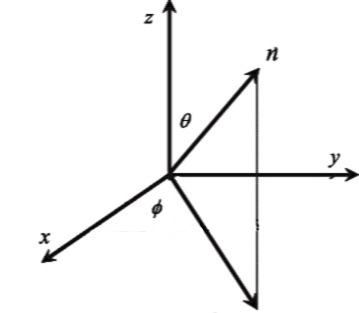
\includegraphics[width=0.8\textwidth]{spherical_harmonics_graph.jpg}
\caption{The image above shows the representation of where $\theta$ and $\phi$ are in relation to a graph.}
\end{figure}

$\theta$ is the co-latitutde and ranges from $0 \leq \theta \leq \pi$ where $0$ is the north pole and $\pi$ is the south pole. 

$\phi$ is the longitute and ranges from $0 \leq \phi \leq 2\pi$.

Let $\mu = \cos(\theta)$. Then $\mu \in [-1,1]$ where $-1$ corresponds to the south pole and $1$ corresponds to the north pole.

\begin{align*}
Y^m _l (\mu, \phi) = \sqrt{\frac{(2l+1)(l-m)!}{4\pi (l+m)!}} P^m _l (\mu) e^{im\phi} \\
\text{Where} P^m _l (\mu) \text{is the associated Legendre function.} \\
\text{Note: } Y^m _l = (-1)^m Y^{-m} _l \\
\end{align*}

\begin{align*}
\text{Let} F(t, \vec{x}, \vec{\Omega}) &= \sum^{\infty}_{l=0} \sum^{l}_{m=-l}  F^m _l (t, \vec{x}) Y^m _l (\mu, \phi) \\
F(t, \vec{x}, \vec{\Omega} &\approx \sum^{N}_{l=0} \sum^{l}_{m=-l} F^m _l (t, \vec{x}) Y^m _l (\mu, \phi)
\end {align*}

The plan is to use spherical harmonics because they are orthonormal on the unit sphere:
\begin{align*}
\int_{s^2} Y^m _l (\mu, \phi) Y^{m'} _{l'} (\mu, \phi) d\vec{\Omega} = \int_{m m'} \int_{l l'}
\end{align*}

Plug $F(t, \vec{x}, \vec{\Omega} \approx \sum^{N}_{l=0} \sum^{l}_{m=-l} F^m _l (t, \vec{x}) Y^m _l (\mu, \phi)$ into the radiative transfer equation, then multiply by $Y^{m'} _{l'}$ then integrate over the unit sphere. Then, after lots of algebra, you are left with linear hyperbolic equations. \\

Let 
\begin{align*}
\vec{F} := (F^0 _0, F^0 _1, F^0 _2, \dots , F^0 _N, F^1 _1, F^1 _2, F^1 _N, \dots , F^N _N)
\end{align*}

Note: These are all functions, $F^m _l (t, \vec{x})$.

Not all functions are in the list since there is some symmetry in the coefficients mentioned above. The unknown coefficients are as follows:

\begin{align*}
l = 0 \quad & F^0 _0 \\
l = 1 \quad & F^0 _1 \quad F^1 _1 \\
l = 2 \quad & F^0 _2 \quad F^1 _2 \quad F^2 _2 \\
l = 3 \quad & F^0 _3 \quad F^1 _3 \quad F^2 _3 \quad F^3 _3 \\
l = 4 \quad & F^0 _4 \quad F^1 _4 \quad F^2 _4 \quad F^3 _4 \quad F^4 _4
\end{align*}

The total number of unknowns is:
\begin{align*}
\sum^N _{l=0} \sum^l _{m=0} i = \frac{1}{2} (N^2 + 3N) + 1 = O(N^2)
\end{align*}